\section{Результаты}
\subsection{Линейный случай}
В качестве матрицы предобуславливания, как это принято, возьмём $\Lambda=(\mathrm{mid}(\textbf{A}))^{-1}$.\\
\subsubsection{Спектральный радиус}
Проверим условие сходимости метода 
\begin{equation}
    |I-\Lambda*A|\approx
    \begin{pmatrix}
0  &  0.0426 \\
0  &  0.0638
\end{pmatrix}
\end{equation}
\begin{equation}
     \rho(|I-\Lambda*A|)\approx0.0638
\end{equation}
\subsubsection{Начальное приближение}
Так как условие $\eta=||I-\Lambda*\textbf{A}||_\infty=0.0638\leq 1$ выполняется, мы можем явно вычислить начальное приближение.
\begin{equation}
    \theta=\frac{||\Lambda \textbf{b}||_\infty}{1-\eta}=7.0455\Rightarrow \textbf{x}^0=([3.5227, 10.5682], [3.5227,   10.5682])^T
\end{equation}
\subsubsection{Внешнее множество решений}
\begin{figure}[H]
\centering
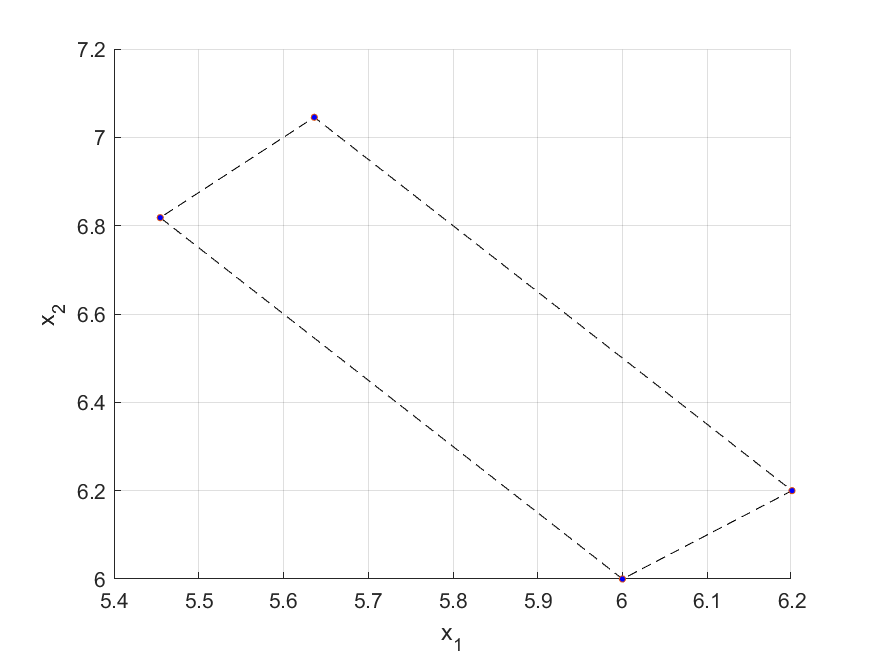
\includegraphics[width=\textwidth]{Graphics/Linear_area.png}
\caption{Внешнее множество решений \eqref{UniSet}} 
\end{figure}
\newpage
\subsubsection{Результаты работы метода}
\begin{figure}[H]
\centering
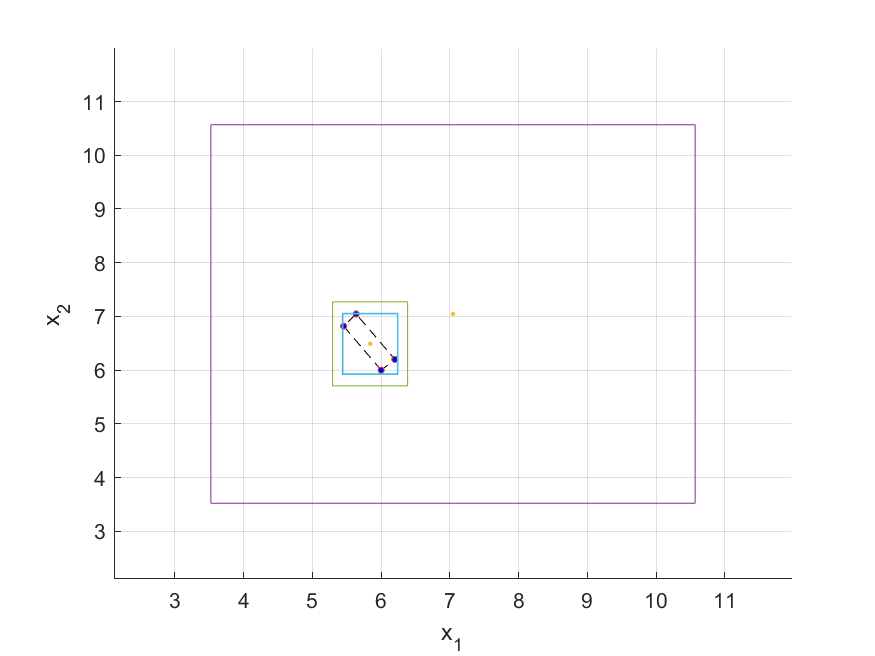
\includegraphics[width=0.9\textwidth]{Graphics/Linear_boxes.png}
\caption{Положения брусов в линейном методе Кравчика} 
\end{figure}
\begin{figure}[H]
\centering
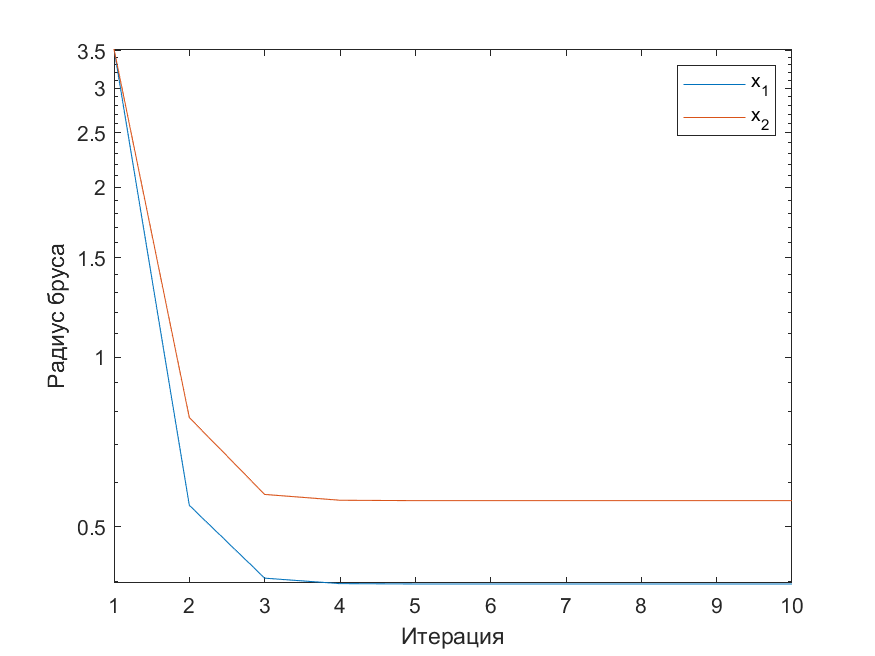
\includegraphics[width=0.9\textwidth]{Graphics/Linear_bar_rad.png}
\caption{Радиусы брусов в линейном методе Кравчика} 
\end{figure}
\begin{figure}[H]
\centering
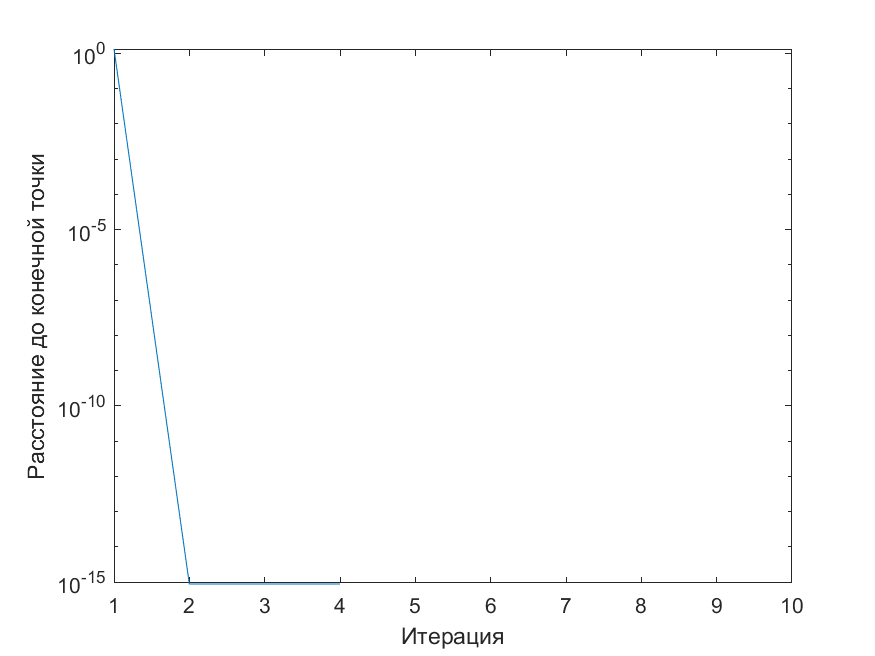
\includegraphics[width=\textwidth]{Graphics/Linear_dist_to_end.png}
\caption{Расстояние до конечного положения в линейном методе Кравчика} 
\end{figure}
\subsection{Нелинейный случай}
Положим интервальную матрицу Липшица $\textbf{L}$ равной якобиану на каждой итерации метода: $\textbf{L}=\textbf{J}(\textbf{X})$.\\
В качестве $\overline{x}^k\in\textbf{X}^k$ будем использовать $\mathrm{mid}(\textbf{X}^k)$.\\
В тоже время определим матрицу предобуславливания как
\begin{equation}
\Lambda(\textbf{X}^k)=(J(\overline{x}^k))^{-1}
\end{equation}
\subsubsection{Спектральный радиус}
Проверим условие сходимости метода 
\begin{equation}
    |I-\Lambda*J|\approx
    \begin{pmatrix}
0.0800  &  0.2720 \\
0.1200  &  0.4080
\end{pmatrix}
\end{equation}
\begin{equation}
     \rho(|I-\Lambda*A|)\approx0.4880
\end{equation}
\subsubsection{Начальное приближение}
В качестве начального приближения возьмём
\begin{equation}
    \textbf{x}^0=([5, 8],[5, 8])^T
\end{equation}
\newpage
\subsubsection{Результаты работы метода}
\begin{figure}[H]
\centering
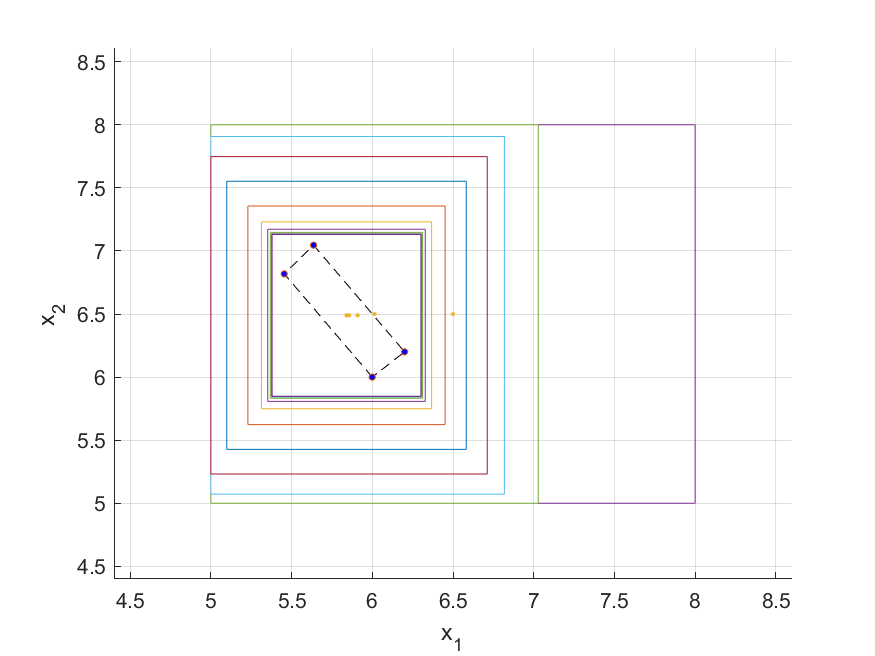
\includegraphics[width=0.9\textwidth]{Graphics/NonLinear_boxes.png}
\caption{Положения брусов в нелинейном методе Кравчика} 
\end{figure}
\begin{figure}[H]
\centering
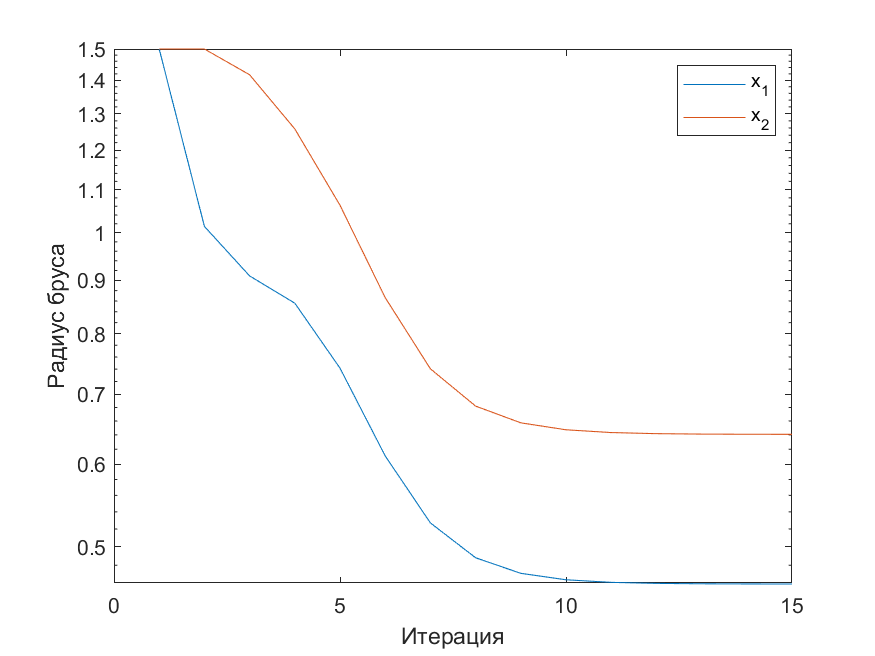
\includegraphics[width=0.9\textwidth]{Graphics/NonLinear_bar_rad.png}
\caption{Радиусы брусов в нелинейном методе Кравчика} 
\end{figure}
\begin{figure}[H]
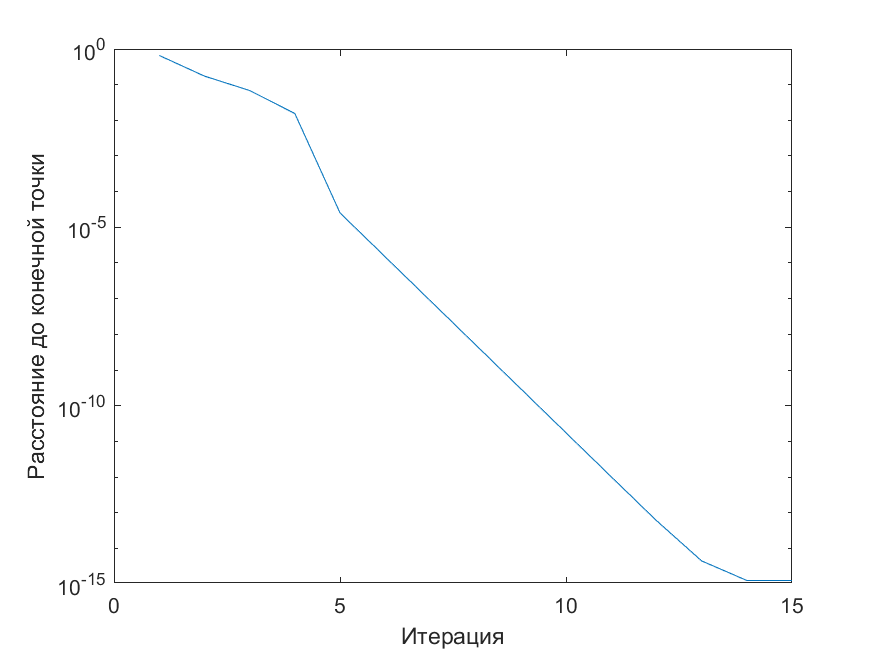
\includegraphics[width=0.9\textwidth]{Graphics/NonLinear_dist_to_end.png}
\caption{Расстояние до конечного положения брусов в нелинейном методе Кравчика} 
\end{figure}
